\graphicspath{{./images},{./monsters/Ebony_Scarab/images}}

\MonsterSheetGeometry

% --------------------------------------------------------------------------------------------------- %
% ################################################################################################### %
% #-#-#-#-#-#-#-#-#-#-#-#-#-#-# Monster-Sheet with two Smaller Pictures #-#-#-#-#-#-#-#-#-#-#-#-#-#-# %
% ################################################################################################### %
% --------------------------------------------------------------------------------------------------- %

\chapter*{Ebony Scarab}
\stepcounter{chapter}
\phantomsection\addcontentsline{toc}{chapter}{\protect\numberline{\thechapter}Ebony Scarab}

\entryfont \noindent \DndDropCapLine{H}ailing from the depths of arid deserts and sun-scorched wastelands, the Ebony Scarab is a marvel of natural engineering. Its chitinous exoskeleton shimmers with a rich hue of black or dark blue, akin to the darkest nights. Yet, this profound darkness is not devoid of life, for intricate golden accents dance across its carapace, capturing the very essence of stardust. These gilded highlights mark its eyes, mandibles, and the fine lines that trace patterns along its armor, a testament to the creature's innate mystique.\\

The Ebony Scarab stands at a formidable 4 to 5 feet in height, its presence radiating an eerie intelligence from its multifaceted, gleaming eyes. Its antennae, in a constant state of delicate twitching, seem to tap into the very vibrations of the earth. As it moves, the sand and soil beneath its feet seem to part willingly, acknowledging the ancient power it wields.\\

This creature's demeanor is a fascinating blend of the graceful and the fearsome. It carries itself with an almost regal bearing, its plated limbs moving with a fluid grace that belies its size. Yet, its mandibles, powerful enough to crush stone and bone alike, provide a constant reminder of its primal nature. When it locks eyes with its prey, an unsettling aura envelops its gaze, capable of instilling terror in even the most resolute souls.\\

Amidst the barren landscapes it calls home, the Ebony Scarab is a master of camouflage. Its exoskeleton, versatile as an artist's palette, can morph to match its surroundings—vanishing into shadows, or blending seamlessly with sand and rock. This natural gift, combined with its keen senses, makes it a predator that strikes from hidden lairs and buried tunnels.

\MonsterGraphicAndShortInfo[shortinfobox=true]% shortinfo or none for no Short-Info Box
{%
	{-8cm}% Shift Horizontal Short Info Box
	{5.5cm}% Shift Vertical Short Info Box
	{25}% Rotation Angle Short Info Box
	{4.5cm}% Width of Short-Info Box
	{6}% Number of Lines in Textbox (might be adjusted after 1 compile) 
	{%
		A meeting with the Ebony Scarab, whether beneath the sun's unforgiving gaze or the starlit canopy of night, is an encounter with the mysteries of the desert - majestic, deadly, and filled with the allure of the unknown.%
	}%
}%
{-0.25cm}% Shift Horizontal Monster Graphic
{0.05cm}% Shift Vertical Monster Graphic
{, anchor=south west}% Further Picture Placement Options
{(current page.south west)}% Anchor-Point on Page
{height=300pt, width=1.5\textwidth}% Dimension of Graphic
{Ebony_Scarab.png}%
\addImageDBEntry{EbonyScarab1}% Handle for the page reference, must be individual for each image
	{Page \thepage}% Display for page numbering. No need for change
	{Monster Art}% more accurate Identifer (BAckground Art, Variant Art, etc.)
	{https://www.deviantart.com/yirikus/art/Ancient-Beetle-Guardian-892850845}% URL to picture or graphic
	{Ancient Beetle Guardian}% Name of Art
	{Yirikus}% Artist

\vfill\eject % cammand to break to next column

\vspace*{-3cm}
\begin{center}\begin{tikzpicture}
	\node[inner sep=0pt, outer sep=0pt] {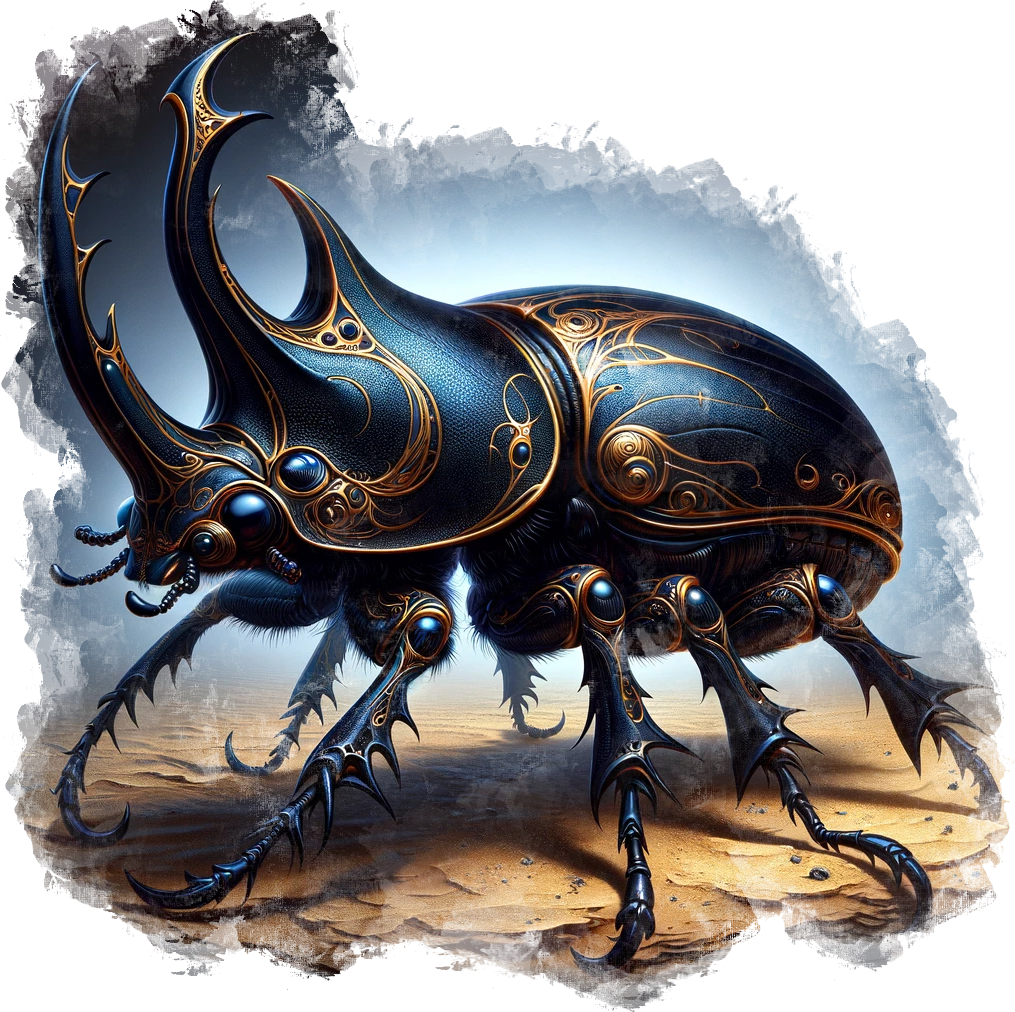
\includegraphics[width=\columnwidth-30pt, keepaspectratio]{Ebony_Scarab(2).png}};
\end{tikzpicture}\end{center}
\vspace*{-1.75cm}
% Monster stat block
\begin{DndMonster}[width=0.5\textwidth]{Ebony Scarab}
    \DndMonsterType{Medium Monstrosity, neutral}

    % If you want to use commas in the key values, enclose the values in braces.
    \DndMonsterBasics[
        armor-class = {15 (Natural Armor)},
        hit-points  = {\DndDice{6d8 + 18}},
        speed       = {30 ft., burrow 20 ft.},
    ]
    
	\renewcommand{\AbilityScoreSpacer}{~}
    \DndMonsterAbilityScores[
		str = 16,
		dex = 14,
		con = 16,
		int = 6,
		wis = 12,
		cha = 7,
    ]

    \DndMonsterDetails[
        %saving-throws = {Str +0, Dex +0, Con +0, Int +0, Wis +0, Cha +0},
        skills = {Perception +3, Stealth +4},
        %damage-vulnerabilities = {cold},
        %damage-resistances = {bludgeoning, piercing, and slashing from nonmagical attacks},
        damage-immunities = {poison},
        senses = {Darkvision 60 ft., Tremorsense 30 ft., Passive Perception 13},
        condition-immunities = {poisoned},
        %languages = {-},
        challenge = 2,
    ]
    
    \DndMonsterAction{Chitinous Armor}
    The Ebony Scarab has a +3 bonus to its Armor Class due to its tough exoskeleton.
	
	\DndMonsterSection{Actions}	
	\DndMonsterAttack[
      name=Crushing Mandibles,
      distance=melee, % valid options are in the set {both,melee,ranged},
      %type=weapon, %valid options are in the set {weapon,spell}
      mod=+5,
      reach=5,
      %range=20/60,
      targets=one target,
      dmg=\DndDice{1d10 + 3},
      dmg-type=slashing,
      %plus-dmg=,
      %plus-dmg-type=,
      %or-dmg=,
      %or-dmg-when=,
      %extra=,
    ]
    
	\DndMonsterAction{Eerie Gaze}
	The Ebony Scarab targets one creature it can see within 30 feet of it. The target must succeed on a DC 13 Wisdom saving throw or be frightened until the end of its next turn.
	
	\DndMonsterAttack[
      name=Infectious Sting,
      distance=melee, % valid options are in the set {both,melee,ranged},
      %type=weapon, %valid options are in the set {weapon,spell}
      mod=+2,
      reach=5,
      %range=20/60,
      targets=one target,
      %dmg=,
      %dmg-type=slashing,
      %plus-dmg=,
      %plus-dmg-type=,
      %or-dmg=,
      %or-dmg-when=,
      extra={The target must make a DC 12 Constitution saving throw or be paralyzed for 1 minute. The target can repeat the saving throw at the end of each of its turns, ending the effect on a success},
    ]
	
	\DndMonsterSection{Reactions}
	\DndMonsterAction{Chromatic Shift}
	When a creature targets the Ebony Scarab with an attack, the scarab can use its reaction to shift its color, imposing disadvantage on the attack roll.
	
\end{DndMonster}